% EOCE Deletions:
% 2.22 and 2.23 were deleted (one on transformations, the other on mapping)
% 2.27 and 2.28 on mosaic plots



\section{Exercises}

%_________________
\subsection{Examining numerical data}

% 1

\eoce{\qt{Mammal life spans} Data were collected on life spans (in years) and gestation lengths (in days) for 62 mammals. A scatterplot of life span versus length of gestation is shown below. \footfullcite{Allison+Cicchetti:1975}

\noindent\begin{minipage}[c]{0.5\textwidth}
\begin{parts}
\item What type of an association is apparent between life span and length of gestation?
\item What type of an association would you expect to see if the axes of the plot were reversed, i.e. if we plotted length of gestation versus life span?
\item Are life span and length of gestation independent? Explain your reasoning.
\end{parts} \vspace{9mm}
\end{minipage}
\begin{minipage}[c]{0.5\textwidth}
\begin{center}
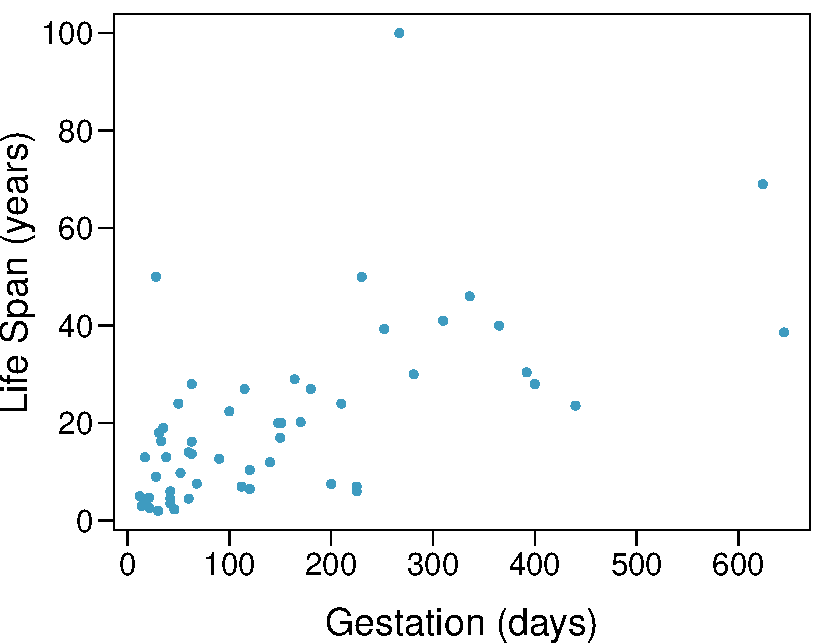
\includegraphics[width = 60mm]{02/figures/eoce/mammals/mammals_lifeSpanGest}
\end{center}
\end{minipage}
}{}


% 2

\eoce{\qt{Office productivity} Office productivity is relatively low when the employees feel no stress about their work or job security. However, high levels of stress can also lead to reduced employee productivity. Sketch a plot to represent the relationship between stress and productivity.
}{}


% 3

\eoce{\qt{Associations} Indicate which of the plots show a \\[1mm]
\noindent\begin{minipage}[b]{0.35\textwidth}
\begin{parts}
\item positive association
\item negative association
\item no association
\end{parts}
Also determine if the positive and negative associations are linear or nonlinear. Each part may refer to more than one plot. \vspace{31mm}
\end{minipage}%
\begin{minipage}[b]{0.62\textwidth}
\hfill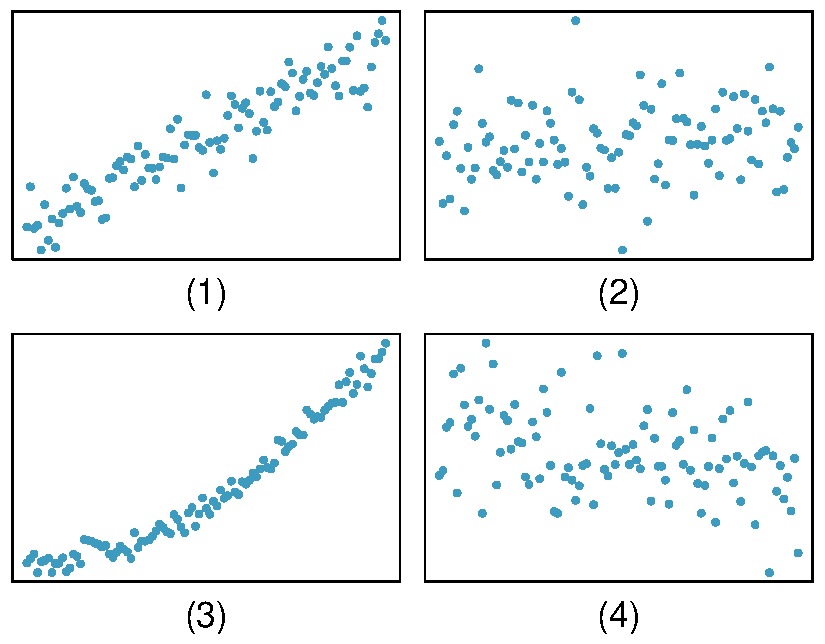
\includegraphics[width = 0.95\textwidth]{02/figures/eoce/associationPlots/associationPlots}
\end{minipage}
}{}



% 4

\eoce{\qt{Parameters and statistics} Identify which value represents the sample mean and which value represents the claimed population mean.
\begin{parts}
\item A recent article in a college newspaper stated that college students get an average of 5.5 hrs of sleep each night. A student who was skeptical about this value decided to conduct a survey by randomly sampling 25 students. On average, the sampled students slept 6.25 hours per night.
\item American households spent an average of about \$52 in 2007 on Halloween merchandise such as costumes, decorations and candy. To see if this number had changed, researchers conducted a new survey in 2008 before industry numbers were reported. The survey included 1,500 households and found that average Halloween spending was \$58 per household.
\item The average GPA of students in 2001 at a private university was 3.37. A survey on a sample of 203 students from this university yielded an average GPA of 3.59 in Spring semester of 2012.
\end{parts}
}{}



\subsection{Numerical summaries and box plots}

% 5

\eoce{\qt{Make-up exam} In a class of 25 students, 24 of them took an exam in class and 1 student took a make-up exam the following day. The professor graded the first batch of 24 exams and found an average score of 74 points with a standard deviation of 8.9 points. The student who took the make-up the following day scored 64 points on the exam.
\begin{parts}
\item Does the new student's score increase or decrease the average score?
\item What is the new average?
\item Does the new student's score increase or decrease the standard deviation of the scores?
\end{parts}
}{}


% 6

\eoce{\qt{Days off at a mining plant} Workers at a particular mining site receive an average of 35 days paid vacation, which is lower than the national average. The manager of this plant is under pressure from a local union to increase the amount of paid time off. However, he does not want to give more days off to the workers because that would be costly. Instead he decides he should fire 10 employees in such a way as to raise the average number of days off that are reported by his employees. In order to achieve this goal, should he fire employees who have the most number of days off, least number of days off, or those who have about the average number of days off?
}{}


% 7

\eoce{\qt{Smoking habits of UK residents, Part I\label{UKSmoking_amounts}} Exercise~\ref{UKSmoking_datamatrix} introduces a data set on the smoking habits of UK residents. Below are histograms displaying the distributions of the number of cigarettes smoked on weekdays and weekends, excluding non-smokers. Describe the two distributions and compare them.
\begin{center}
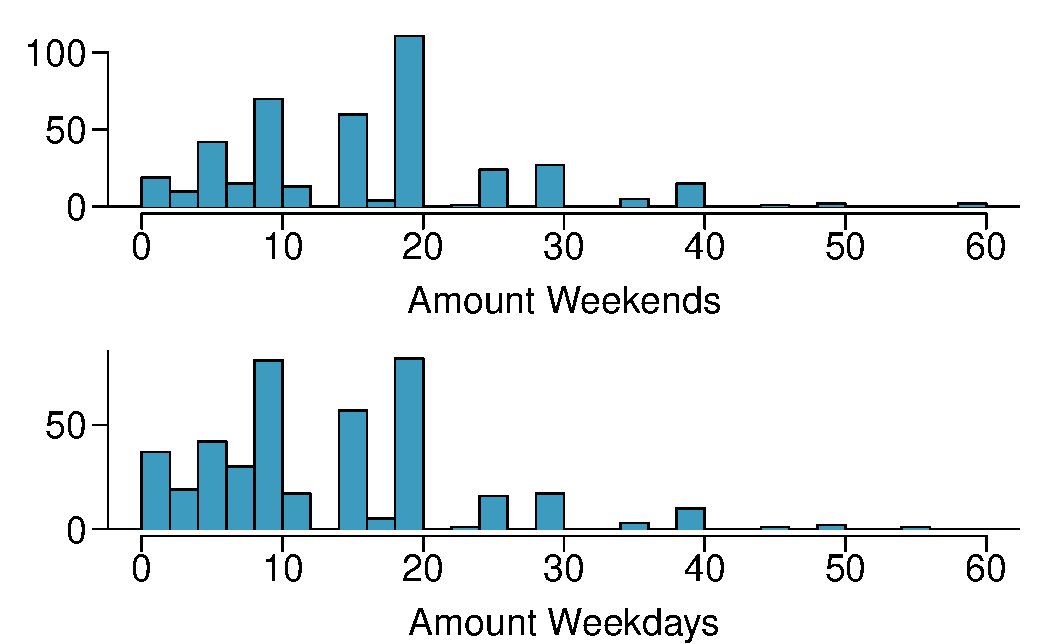
\includegraphics[width = 0.7\textwidth]{02/figures/eoce/smoking/smoking_amountHist}
\end{center}
}{}


% 8

\eoce{\qt{Stats scores\label{introStatsFinalScores}} Below are the final scores of 20 introductory statistics students.
\begin{center}
79, 83, 57, 82, 94, 83, 72, 74, 73, 71, \\
66, 89, 78, 81, 78, 81, 88, 69, 77, 79
\end{center}
Draw a histogram of these data and describe the distribution.
}{}


% 9

\eoce{\qt{Smoking habits of UK residents, Part II} A random sample of 5 smokers from the data set discussed in Exercises~\ref{UKSmoking_datamatrix} and \ref{UKSmoking_amounts} is provided below.
{\footnotesize
\begin{center}
\begin{tabular}{ccccccc}
  \hline
gender & age & maritalStatus & grossIncome & smoke & amtWeekends & amtWeekdays \\ 
  \hline
Female &  51 & Married & $\pounds$2,600 to $\pounds$5,200 & Yes &  20 cig/day &  20 cig/day\\ 
  Male &  24 & Single & $\pounds$10,400 to $\pounds$15,600 & Yes &  20 cig/day&  15 cig/day\\ 
  Female &  33 & Married & $\pounds$10,400 to $\pounds$15,600 & Yes &  20 cig/day&  10 cig/day\\ 
  Female &  17 & Single & $\pounds$5,200 to $\pounds$10,400 & Yes &  20 cig/day&  15 cig/day\\ 
  Female &  76 & Widowed & $\pounds$5,200 to $\pounds$10,400 & Yes &  20 cig/day&  20 cig/day\\ 
   \hline
\end{tabular}
\end{center}
}
\begin{parts}
\item Find the mean amount of cigarettes smoked on weekdays and weekends by these 5 respondents.
\item Find the standard deviation of the amount of cigarettes smoked on weekdays and on weekends by these 5 respondents. Is the variability higher on weekends or on weekdays?
\end{parts}
}{}


% 10

\eoce{\qt{Factory defective rate} A factory quality control manager decides to investigate the percentage of defective items produced each day. Within a given work week (Monday through Friday) the percentage of defective items produced was 2\%, 1.4\%, 4\%, 3\%, 2.2\%.
\begin{parts}
\item Calculate the mean for these data.
\item Calculate the standard deviation for these data, showing each step in detail.
\end{parts}
}{}


% 11

\eoce{\qt{Medians and IQRs} For each part, compare distributions (1) and (2) based on their medians and IQRs. You do not need to calculate these statistics; simply state how the medians and IQRs compare. Make sure to explain your reasoning. 
\begin{multicols}{2}
\begin{parts}
\item (1) 3, 5, 6, 7, 9 \\
(2) 3, 5, 6, 7, 20
\item (1) 3, 5, 6, 7, 9 \\
(2) 3, 5, 8, 7, 9
\item (1) 1, 2, 3, 4, 5 \\
(2) 6, 7, 8, 9, 10
\item (1) 0, 10, 50, 60, 100 \\
(2) 0, 100, 500, 600, 1000
\end{parts}
\end{multicols}
}{}


% 12

\eoce{\qt{Means and SDs} For each part, compare distributions (1) and (2) based on their means and standard deviations. You do not need to calculate these statistics; simply state how the means and the standard deviations compare. Make sure to explain your reasoning. \textit{Hint:} It may be useful to sketch dot plots of the distributions.
\begin{multicols}{2}
\begin{parts}
\item (1) 3, 5, 5, 5, 8, 11, 11, 11, 13 \\
(2) 3, 5, 5, 5, 8, 11, 11, 11, 20 \\
\item (1) -20, 0, 0, 0, 15, 25, 30, 30 \\
(2) -40, 0, 0, 0, 15, 25, 30, 30
\item (1) 0, 2, 4, 6, 8, 10 \\
(2) 20, 22, 24, 26, 28, 30
\item (1) 100, 200, 300, 400, 500 \\
(2) 0, 50, 300, 550, 600
\end{parts}
\end{multicols}
}{}


% 13

\eoce{\qt{Box plot} Create a box plot for the data given in Exercise~\ref{introStatsFinalScores}. The five number summary provided below may be useful.
\begin{center}
\renewcommand\arraystretch{1.5}
\begin{tabular}{ccccc}
Min	& Q1	& Q2 (Median)	& Q3	& Max \\
\hline
57	& 72.5	& 78.5	& 82.5	& 94 \\
\end{tabular}
\end{center}
}{}


% 14

\eoce{\qt{Infant mortality} The infant mortality rate is defined as the number of infant deaths per 1,000 live births. This rate is often used as an indicator of the level of health in a country. The relative frequency histogram below shows the distribution of estimated infant death rates in 2012 for 222 countries. \footfullcite{data:ciaFactBookInfMort:2012}

\noindent\begin{minipage}[c]{0.43\textwidth}
\begin{parts}
\item Estimate Q1, the median, and Q3 from the histogram.
\item Would you expect the mean of this data set to be smaller or larger than the median? Explain your reasoning.
\end{parts}
\vspace{18mm}
\end{minipage}
\begin{minipage}[c]{0.52\textwidth}
\hfill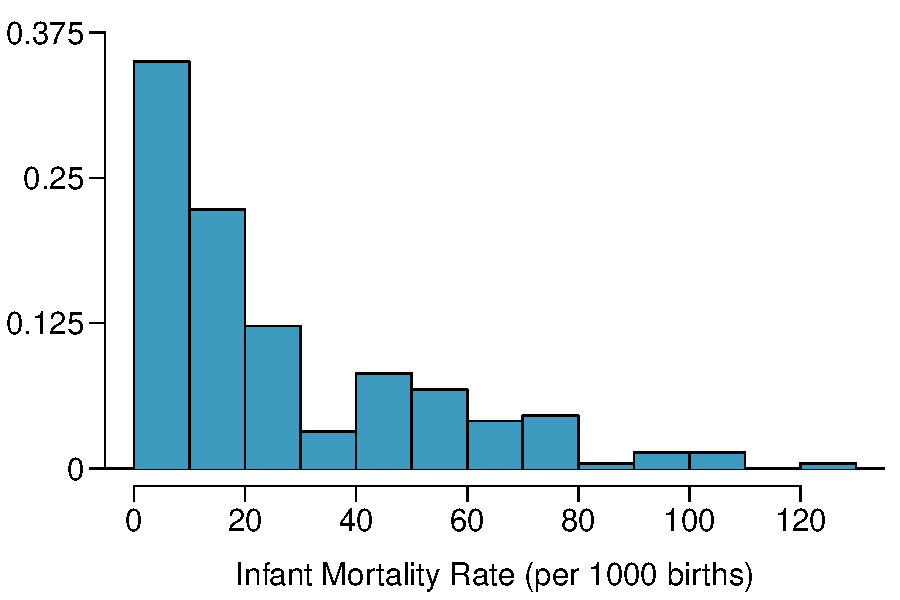
\includegraphics[width = 0.95\textwidth]{02/figures/eoce/country/country_infMort}
\end{minipage}
}{}


% 15

\eoce{\qt{Matching histograms and box plots} Describe the distribution in the histograms below and match them to the box plots. \\
\begin{center}
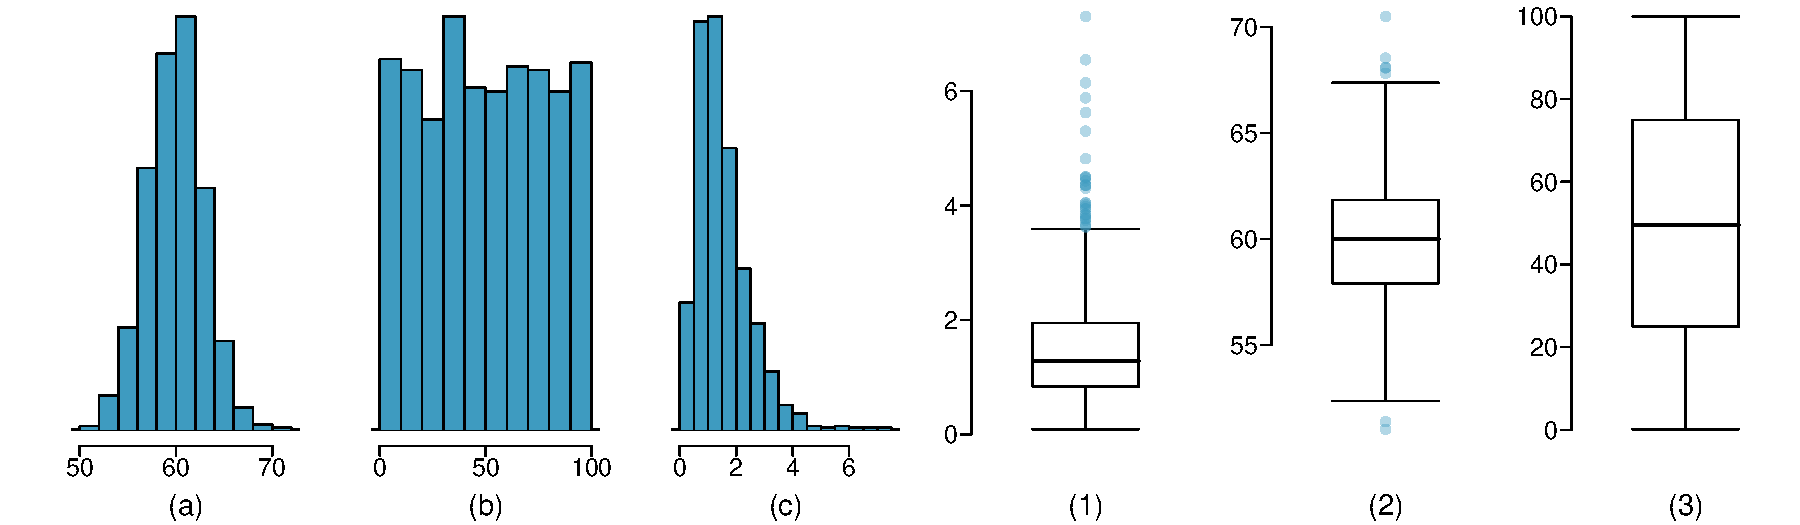
\includegraphics[width =\textwidth]{02/figures/eoce/histBoxMatch/histBoxMatch}
\end{center}
}{}


% 16

\eoce{\qt{Air quality\label{durhamAQI}} Daily air quality is measured by the air quality index (AQI) reported by the Environmental Protection Agency. This index reports the pollution level and what associated health effects might be a concern. The index is calculated for five major air pollutants regulated by the Clean Air Act. and takes values from 0 to 300, where a higher value indicates lower air quality. AQI was reported for a sample of 91 days in 2011 in Durham, NC. The relative frequency histogram below shows the distribution of the AQI values on these days. \footfullcite{data:durhamAQI:2011}
\begin{center}
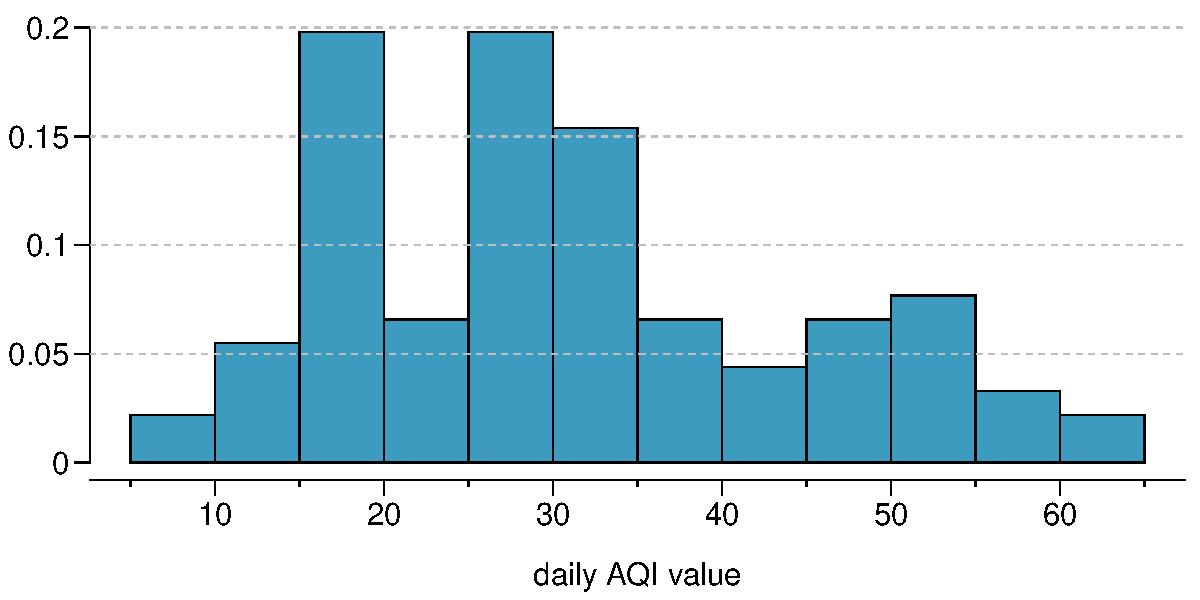
\includegraphics[width = 0.75\textwidth]{02/figures/eoce/durhamAQI/durhamAQI_hist} 
\end{center}
\begin{parts}
\item Estimate the median AQI value of this sample.
\item Would you expect the mean AQI value of this sample to be higher or lower than the median? Explain your reasoning.
\item Estimate Q1, Q3, and IQR for the distribution.
\end{parts}
}{}


% 17

\eoce{\qt{Histograms and box plots} Compare the two plots below. What characteristics of the distribution are apparent in the histogram and not in the box plot? What characteristics are apparent in the box plot but not in the histogram?
\begin{center}
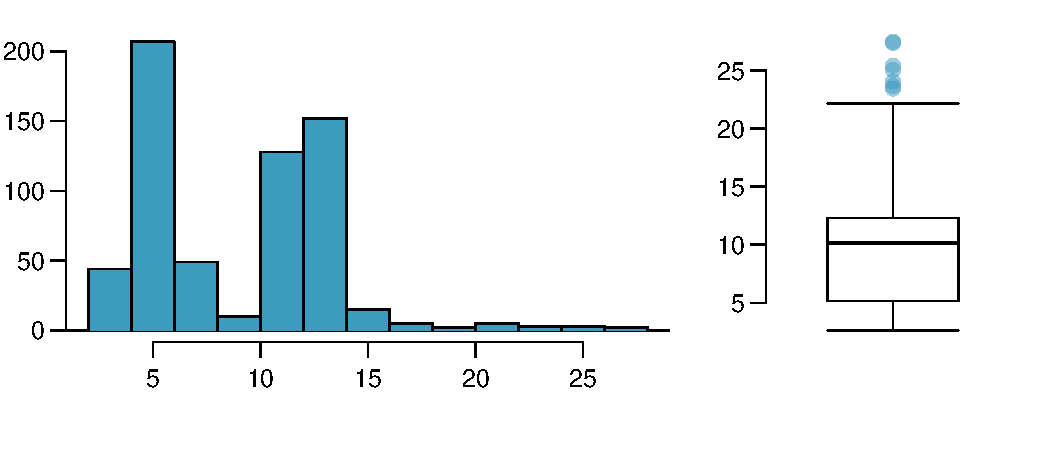
\includegraphics[width = 0.77\textwidth]{02/figures/eoce/bimodalHistBox/bimodalHistBox}
\end{center}
}{}


% 18

\eoce{\qt{Marathon winners\label{NYMarathon}} The histogram and box plots below show the distribution of finishing times for male and female winners of the New York Marathon between 1970 and 1999.
\begin{center}
\includegraphics[width=0.9\textwidth]{02/figures/eoce/marathon/marathon_histBox}
\end{center}
\begin{parts}
\item What features of the distribution are apparent in the histogram and not the box plot? What features are apparent in the box plot but not in the histogram?
\item What may be the reason for the bimodal distribution? Explain.
\item Compare the distribution of marathon times for men and women based on the box plot shown below.
\begin{center}
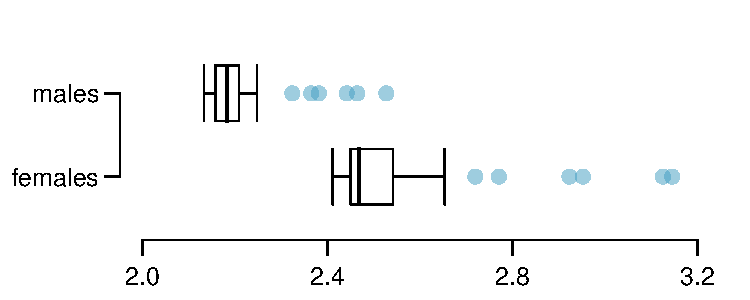
\includegraphics[width=0.7\textwidth]{02/figures/eoce/marathon/marathon_genderBox}
\end{center}
\item The time series plot shown below is another way to look at these data. Describe what is visible in this plot but not in the others.
\end{parts}
\begin{center}
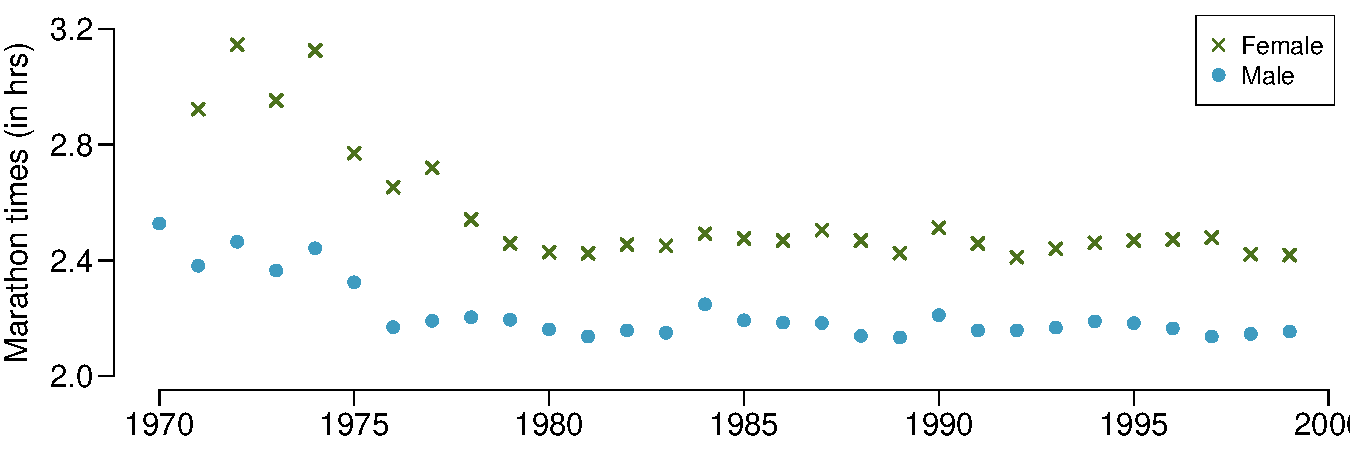
\includegraphics[width=0.95\textwidth]{02/figures/eoce/marathon/marathon_genderTimeSeries} \\
\end{center}
}{}


% 19

\eoce{\qt{Robust statistics} The first histogram below shows the distribution of the yearly incomes of 40 patrons at a college coffee shop. Suppose two new people walk into the coffee shop: one making \$225,000 and the other \$250,000. The second histogram shows the new income distribution. Summary statistics are also provided. \\
\begin{minipage}[c]{0.57\textwidth}
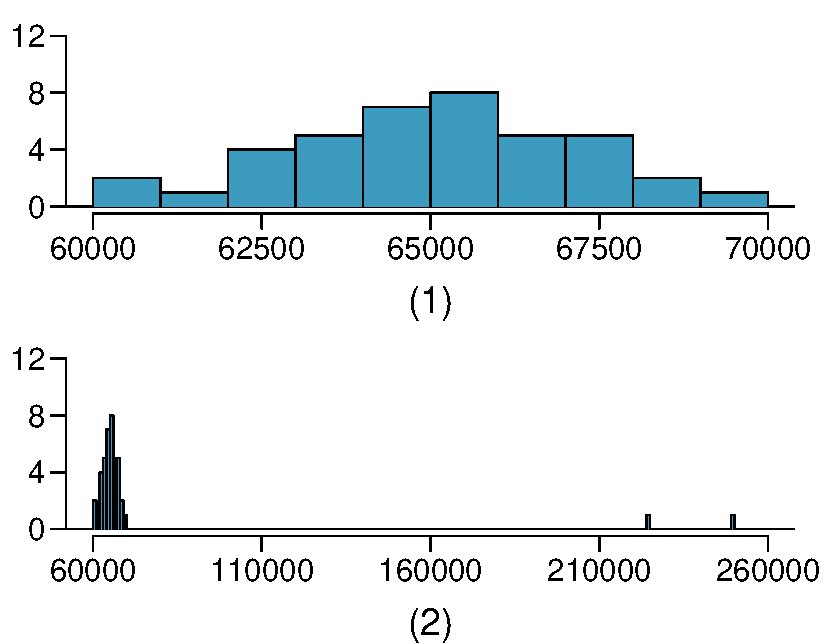
\includegraphics[width=\textwidth]{02/figures/eoce/salary/salary}
\end{minipage}
\begin{minipage}[c]{0.4\textwidth}
\begin{center}
\begin{tabular}{rrr}
  \hline
 & (1) & (2) \\ 
  \hline
n & 40 & 42 \\ 
  Min. & 60,680 & 60,680 \\ 
  1st Qu. & 63,620 & 63,710 \\ 
  Median & 65,240 & 65,350 \\ 
  Mean & 65,090 & 73,300 \\ 
  3rd Qu. & 66,160 & 66,540 \\ 
  Max. & 69,890 & 250,000 \\ 
  SD & 2,122 & 37,321 \\ 
   \hline
\end{tabular}
\end{center}
\end{minipage}
\begin{parts}
\item Would the mean or the median best represent what we might think of as a typical income for the 42 patrons at this coffee shop? What does this say about the robustness of the two measures?
\item Would the standard deviation or the IQR best represent the amount of variability in the incomes of the 42 patrons at this coffee shop? What does this say about the robustness of the two measures?
\end{parts}
}{}


% 20

\eoce{\qt{Distributions and appropriate statistics} For each of the following, describe whether you expect the distribution to be symmetric, right skewed, or left skewed. Also specify whether the mean or median would best represent a typical observation in the data, and whether the variability of observations would be best represented using the standard deviation or IQR.
\begin{parts}
\item Housing prices in a country where 25\% of the houses cost below \$350,000, 50\% of the houses cost below \$450,000, 75\% of the houses cost below \$1,000,000 and there are a meaningful number of houses that cost more than \$6,000,000.
\item Housing prices in a country where 25\% of the houses cost below \$300,000, 50\% of the houses cost below \$600,000, 75\% of the houses cost below \$900,000 and very few houses that cost more than \$1,200,000.
\item Number of alcoholic drinks consumed by college students in a given week.
\item Annual salaries of the employees at a Fortune 500 company.
\end{parts}
}{}


% 21

\noindent\begin{minipage}[c]{0.4\textwidth}
\eoce{\qt{Commuting times, Part I\label{workTravel}} The histogram to the right shows the distribution of mean commuting times in 3,143 US counties in 2010. Describe the distribution and comment on whether or not a log transformation may be advisable for these data.
}{} \vspace{5mm}
\end{minipage}%
\begin{minipage}[c]{0.58\textwidth}
\begin{center}
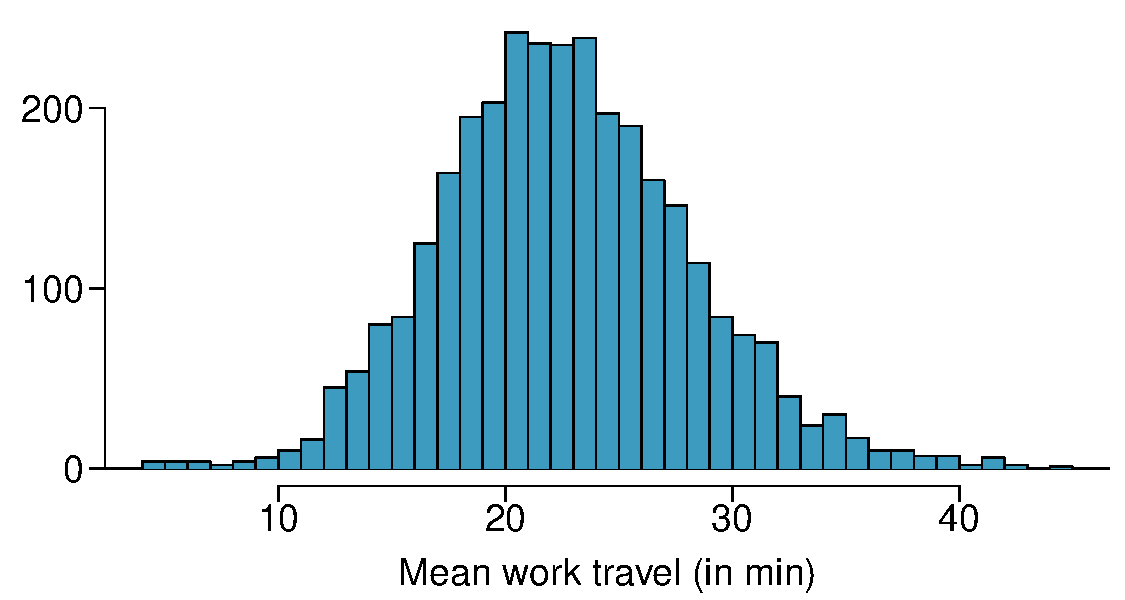
\includegraphics[width=\textwidth]{02/figures/eoce/county/county_workTravelHist}
\end{center}
\end{minipage}


% 22 (22 & 23 deleted)

\eoce{\qt{Hispanic population} The map below  shows the distribution of the percentage of the population that is Hispanic in 3,143 counties in the US in 2010. Explain why it the map would be more helpful than a histogram of the percentages.
\begin{center}
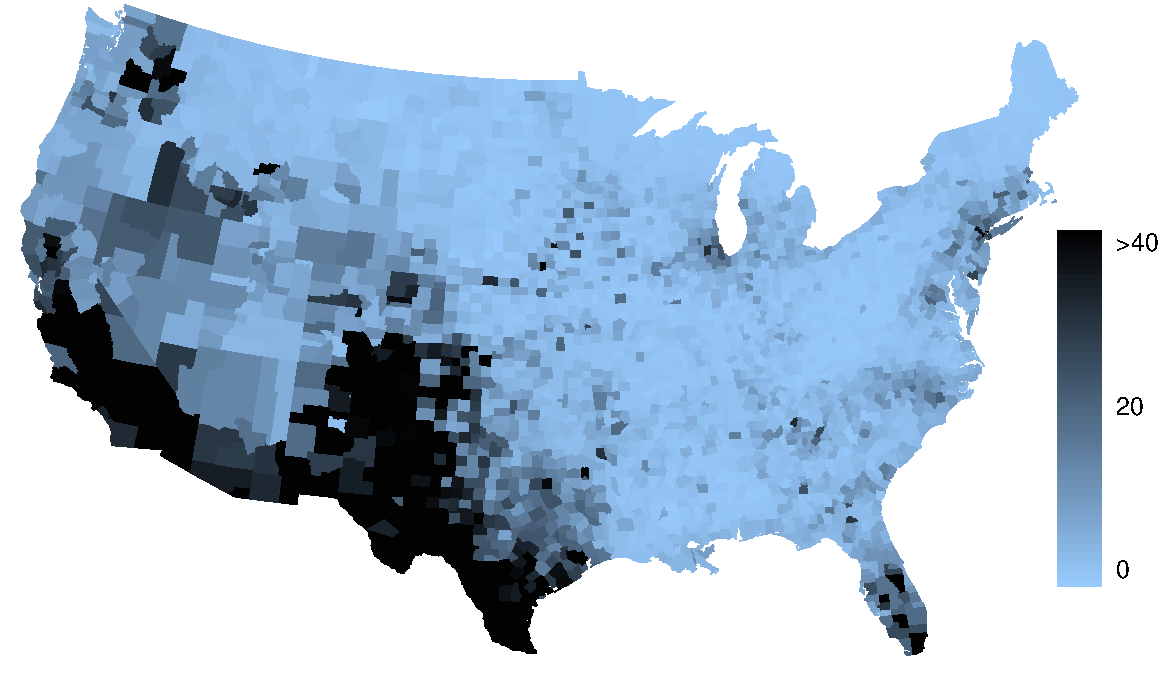
\includegraphics[width=\textwidth]{02/figures/eoce/county/county_hispMap}
\end{center}
}{}


%_________________
\subsection{Considering categorical data}

% 23

\eoce{\qt{Antibiotic use in children} The bar plot and the pie chart below show the distribution of pre-existing medical conditions of children involved in a study on the optimal duration of antibiotic use in treatment of tracheitis, which is an upper respiratory infection.
\begin{parts}
\item What features are apparent in the bar plot but not in the pie chart?
\item What features are apparent in the pie chart but not in the bar plot?
\item Which graph would you prefer to use for displaying these categorical data?
\end{parts}
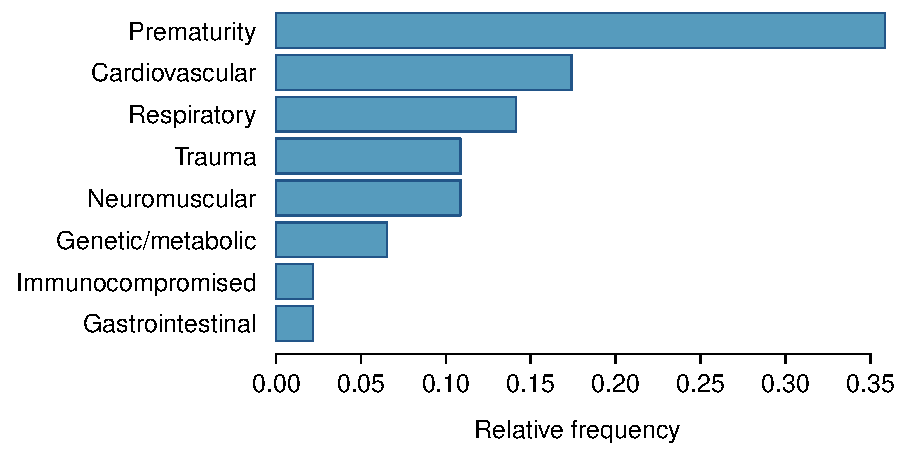
\includegraphics[width = 0.6\textwidth]{02/figures/eoce/tracheitis/tracheitis_bar}
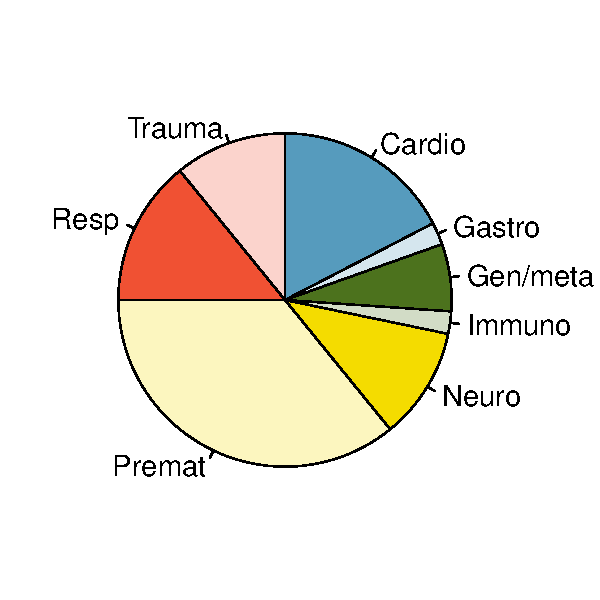
\includegraphics[width = 0.35\textwidth]{02/figures/eoce/tracheitis/tracheitis_pie}
}{}


% 24

\eoce{\qt{Views on immigration\label{immigration}} 910 randomly sampled registered voters from Tampa, FL were asked if they thought workers who have illegally entered the US should be (i) allowed to keep their jobs and apply for US citizenship, (ii) allowed to keep their jobs as temporary guest workers but not allowed to apply for US citizenship, or (iii) lose their jobs and have to leave the country. The results of the survey by political ideology are shown below.\footfullcite{survey:immigFL:2012}
\begin{center}
\begin{tabular}{l l  c c c c}
				&		& \multicolumn{3}{c}{\textit{Political ideology}} \\
\cline{3-5}
				& & Conservative	& Moderate	& Liberal 	& Total \\
\cline{2-6}
& (i) Apply for citizenship	& 57			& 120		& 101	& 278 \\
& (ii) Guest worker		& 121		& 113		& 28		& 262 \\
\raisebox{1.5ex}[0pt]{\emph{Response}} &(iii) Leave the country	& 179		& 126		& 45		& 350 \\ 
& (iv) Not sure			& 15			& 4			& 1		& 20\\
\cline{2-6}
& Total				& 372		& 363		& 175	& 910
\end{tabular}
\end{center}
\begin{parts}
\item What percent of these Tampa, FL voters identify themselves as conservatives?
\item What percent of these Tampa, FL voters are in favor of the citizenship option?
\item What percent of these Tampa, FL voters identify themselves as conservatives and are in favor of the citizenship option?
\item What percent of these Tampa, FL voters who identify themselves as conservatives are also in favor of the citizenship option? What percent of moderates and liberal share this view?
\item Do political ideology and views on immigration appear to be independent? Explain your reasoning.
\end{parts}
}{}



%_________________
\subsection{Case study: gender discrimination}

% 27

\eoce{\qt{Side effects of Avandia, Part I\label{AvandiaTrueFalse}} Rosiglitazone is the active ingredient in the controversial type~2 diabetes medicine Avandia and has been linked to an increased risk of serious cardiovascular problems such as stroke, heart failure, and death. A common alternative treatment is pioglitazone, the active ingredient in a diabetes medicine called Actos. In a nationwide retrospective observational study of 227,571 Medicare beneficiaries aged  65 years or older, it was found that 2,593 of the 67,593 patients using rosiglitazone and 5,386 of the 159,978 using pioglitazone had serious cardiovascular problems. These data are summarized in the contingency table below. \footfullcite{Graham:2010}
\begin{center}
\begin{tabular}{ll  cc c} 
								&				& \multicolumn{2}{c}{\textit{Cardiovascular problems}} \\
\cline{3-4}	
								&				& Yes 	& No 		& Total	\\
\cline{2-5}
\multirow{2}{*}{\textit{Treatment}}		& Rosiglitazone 	& 2,593	& 65,000		& 67,593 	\\
								& Pioglitazone		& 5,386 	& 154,592 	& 159,978\\
\cline{2-5}
								&Total			& 7,979	& 219,592		& 227,571
\end{tabular}
\end{center}
Determine if each of the following statements is true or false. If false, explain why. \textit{Be careful:} The reasoning may be wrong even if the statement's conclusion is correct. In such cases, the statement should be considered false.
\begin{parts}
\item Since more patients on pioglitazone had cardiovascular problems (5,386 vs. 2,593), we can conclude that the rate of cardiovascular problems for those on a pioglitazone treatment is higher.
\item The data suggest that diabetic patients who are taking rosiglitazone are more likely to have cardiovascular problems since the rate of incidence was (2,593 / 67,593 = 0.038) 3.8\% for patients on this treatment, while it was only (5,386 / 159,978 = 0.034) 3.4\% for patients on pioglitazone.
\item The fact that the rate of incidence is higher for the rosiglitazone group proves that rosiglitazone causes serious cardiovascular problems.
\item Based on the information provided so far, we cannot tell if the difference between the rates of incidences is due to a relationship between the two variables or due to chance.
\end{parts}
}{}


% 28

\eoce{\qt{Heart transplants} The Stanford University Heart Transplant Study was conducted to determine whether an experimental heart transplant program increased lifespan. Each patient entering the program was designated an official heart transplant candidate, meaning that he was gravely ill and would most likely benefit from a new heart. Some patients got a transplant and some did not. The variable \texttt{transplant} indicates which group the patients were in; patients in the treatment group got a transplant and those in the control group did not. Another variable called \texttt{survived} was used to indicate whether or not the patient was alive at the end of the study. \textB{Figures may be found on the next page.} \footfullcite{Turnbull+Brown+Hu:1974}

Of the 34 patients in the control group, 4 were alive at the end of the study. Of the 69 patients in the treatment group, 24 were alive. The contingency table below summarizes these results.
\begin{center}
\begin{tabular}{ll  cc c} 
							&		& \multicolumn{2}{c}{\textit{Group}} \\
\cline{3-4}
							&		& Control 	& Treatment 	& Total	\\
\cline{2-5}
							& Alive 	& 4	 	& 24			& 28 	\\
\raisebox{1.5ex}[0pt]{\emph{Outcome}} & Dead	& 30		& 45	 		& 75\\
\cline{2-5}
							& Total	& 34		& 69			& 103
\end{tabular}
\end{center}
\begin{parts}
\item What proportion of patients in the treatment group and what proportion of patients in the control group died?
\item One approach for investigating whether or not the treatment is effective is to use a randomization technique.
\begin{subparts}
\item What are the claims being tested?
\item  The paragraph below describes the set up for such approach, if we were to do it without using statistical software. Fill in the blanks with a number or phrase, whichever is appropriate.
\begin{adjustwidth}{2em}{2em}
We write \textit{alive} on \rule{2cm}{0.5pt} cards representing patients who were alive at the end of the study, and \textit{dead} on \rule{2cm}{0.5pt} cards representing patients who were not. Then, we shuffle these cards and split them into two groups: one group of size \rule{2cm}{0.5pt} representing treatment, and another group of size \rule{2cm}{0.5pt} representing control. We calculate the difference between the proportion of \textit{dead} cards in the treatment and control groups (treatment - control) and record this value. We repeat this many times to build a distribution centered at \rule{2cm}{0.5pt}. Lastly, we calculate the fraction of simulations where the simulated differences in proportions are \rule{2cm}{0.5pt}. If this fraction is low, we conclude that it is unlikely to have observed such an outcome by chance and that the null hypothesis (independence model) should be rejected in favor of the alternative.
\end{adjustwidth}
\item What do the simulation results shown below suggest about the effectiveness of the transplant program?
\end{subparts}
\end{parts}
\begin{center}
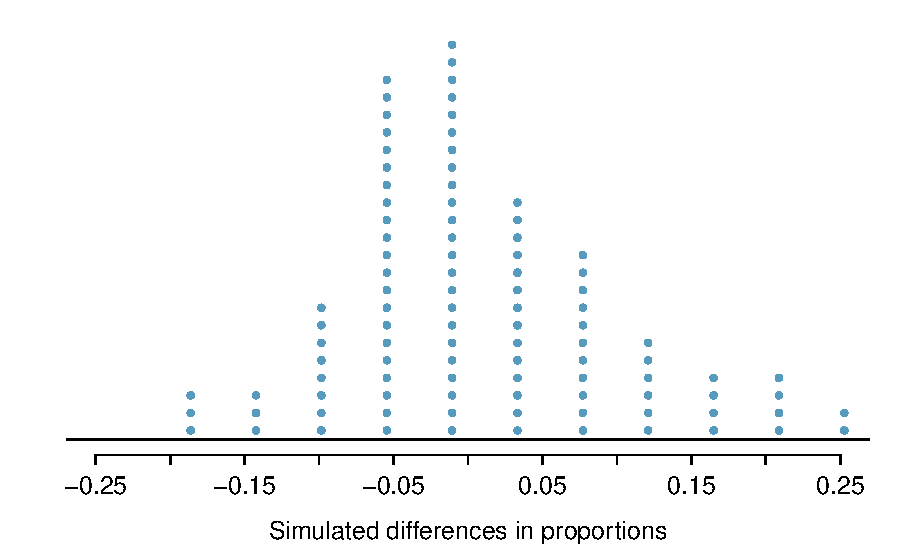
\includegraphics[width = 0.75\textwidth]{02/figures/eoce/heartTr/heartTr_RandHist} \\
\end{center}
}{}


% 29

\eoce{\qt{Side effects of Avandia, Part II} Exercise~\ref{AvandiaTrueFalse} introduces a study that compares the rates of serious cardiovascular problems for diabetic patients on rosiglitazone and pioglitazone treatments. The table below summarizes the results of the study.
\begin{center}
\begin{tabular}{ll  cc c} 
								&				& \multicolumn{2}{c}{\textit{Cardiovascular problems}} \\
\cline{3-4}	
								&				& Yes 	& No 		& Total	\\
\cline{2-5}
\multirow{2}{*}{\textit{Treatment}}		& Rosiglitazone 	& 2,593	& 65,000		& 67,593 	\\
								& Pioglitazone		& 5,386 	& 154,592 	& 159,978\\
\cline{2-5}
								&Total			& 7,979	& 219,592		& 227,571
\end{tabular}
\end{center}
\begin{parts}
\item What proportion of all patients had cardiovascular problems?
\item If the type of treatment and having cardiovascular problems were independent, about how many patients in the rosiglitazone group would we expect to have had cardiovascular problems?
\item We can investigate the relationship between outcome and treatment in this study using a randomization technique.  While in reality we would carry out the simulations required for randomization using statistical software, suppose we actually simulate using index cards. In order to simulate from the independence model, which states that the outcomes were independent of the treatment, we write whether or not each patient had a cardiovascular problem on cards, shuffled all the cards together, then deal them into two groups of size 67,593 and 159,978. We repeat this simulation 1,000 times and each time record the number of people in the rosiglitazone group who had cardiovascular problems. Below is a relative frequency histogram of these counts. \\
\begin{subparts}
\item What are the claims being tested?
\item Compared to the number calculated in part (b), which would provide more support for the alternative hypothesis,  \textit{more} or \textit{fewer} patients with cardiovascular problems in the rosiglitazone group?
\item What do the simulation results suggest about the relationship between taking rosiglitazone and having cardiovascular problems in diabetic patients?
\end{subparts}
\begin{center}
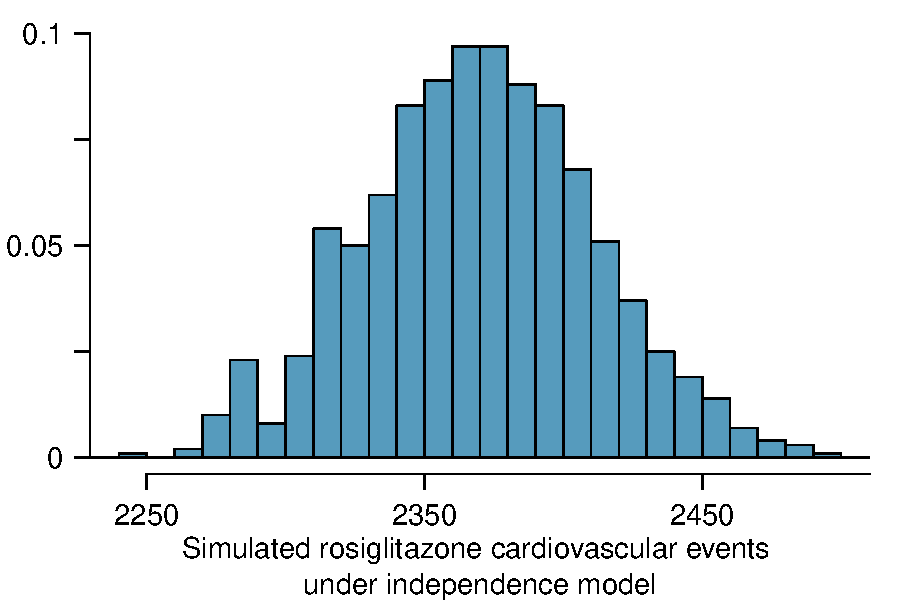
\includegraphics[width = 0.75\textwidth]{02/figures/eoce/avandia/avandia_RandHist} \\
\end{center}
\end{parts}
}{}


% 30

\eoce{\qt{Sinusitis and antibiotics, Part II} Researchers studying the effect of antibiotic treatment compared to symptomatic treatment for acute sinusitis randomly assigned 166 adults diagnosed with sinusitis into two groups (as discussed in Exercise~\ref{sinusitis}). Participants in the antibiotic group received a 10-day course of an antibiotic, and the rest received symptomatic treatments as a placebo. These pills had the same taste and packaging as the antibiotic. At the end of the 10-day period patients were asked if they experienced improvement in symptoms since the beginning of the study. The distribution of responses is summarized below. \footfullcite{Garbutt:2012}
\begin{center}
\begin{tabular}{ll  cc c} 
			&				& \multicolumn{2}{c}{\textit{Self reported}} \\
			&				& \multicolumn{2}{c}{\textit{improvement in symptoms}} \\
\cline{3-4}
			&							& Yes 	& No 	& Total	\\
\cline{2-5}
							&Antibiotic 	& 66	 	& 19		& 85 	\\
\raisebox{1.5ex}[0pt]{\textit{Treatment}}	& Placebo		& 65	 	& 16 	 	& 81 \\
\cline{2-5}
							&Total		& 131	& 35		& 166
\end{tabular}
\end{center}
\begin{parts}
\item What type of a study is this?
\item Does this study make use of blinding?
\item At first glance, does antibiotic or placebo appear to be more effective for the treatment of sinusitis? Explain your reasoning using appropriate statistics.
\item There are two competing claims that this study is used to compare: the independence model and the alternative model. Write out these competing claims in easy-to-understand language and in the context of the application. \textit{Hint:} The researchers are studying the effectiveness of antibiotic treatment.
\item Based on your finding in (c), does the evidence favor the alternative model? If not, then explain why. If so, what would you do to check if whether this is strong evidence?
\end{parts}
}{}
